\chapter{基于生成对抗网络的图像翻译方法}
\section{生成对抗网络}
\subsection{生成对抗网络原理}
\begin{figure*}[ht]
    \centering
	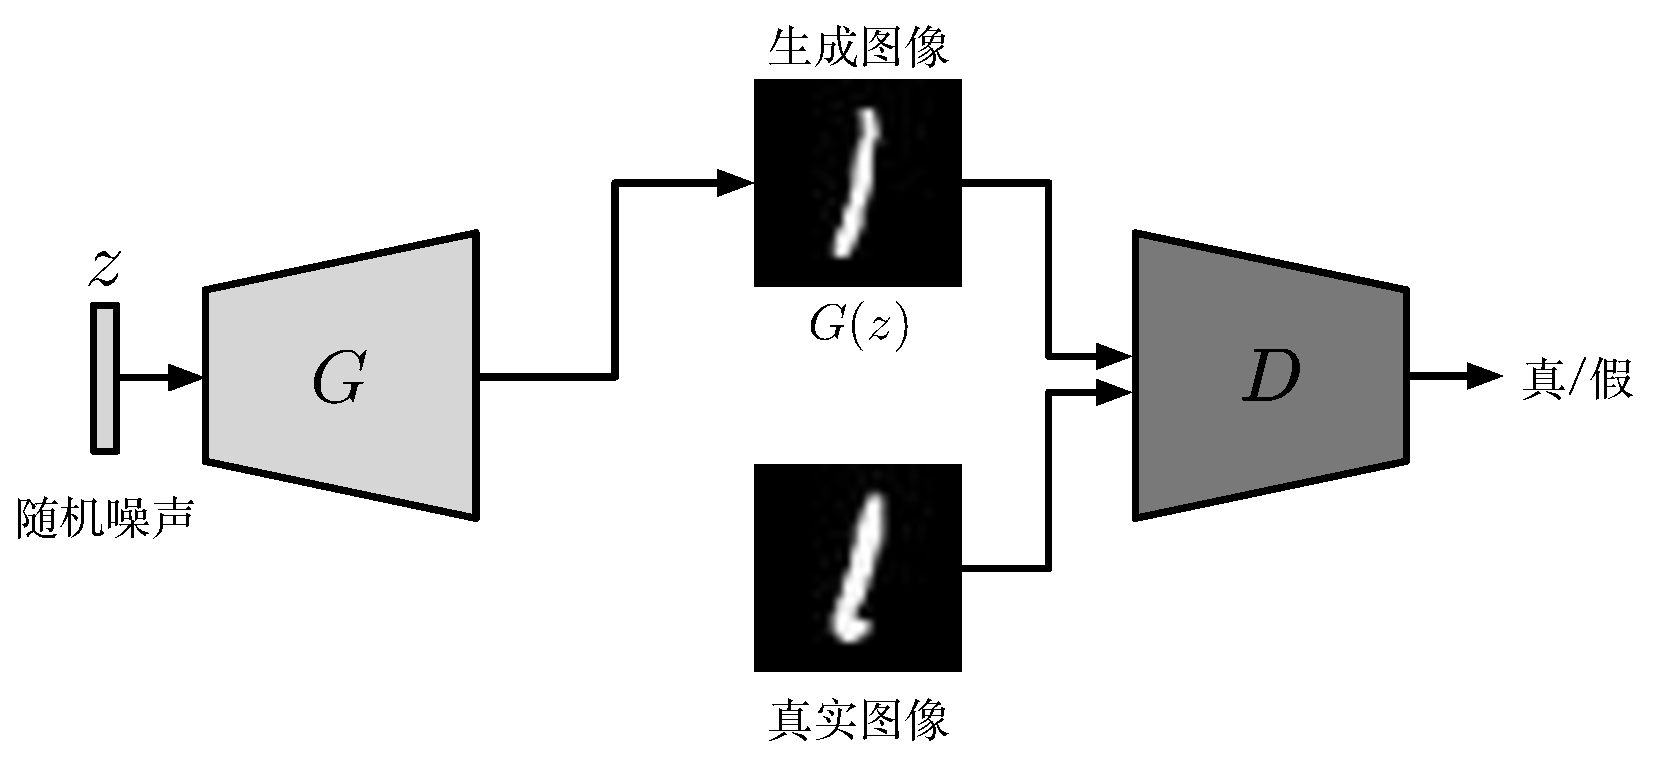
\includegraphics[width=\textwidth]{figures/gan.pdf}
	\caption{生成对抗网络示意图~\cite{goodfellow2014generative}。}
	\label{fig:pic_gan}
\end{figure*}

Goodfellow在2014年提出生成对抗网络(GAN)~\cite{goodfellow2014generative}。生成对抗网络的提出采用二人零和博弈思想,两个神经网络在游戏框架下相互博弈,不断彼此优化,网络结构如图~\ref{fig:pic_gan}所示。由两个彼此独立的神经网络组成:一个生成器$G$,输入随机噪声向量$z$,输出合成数结果据$G(z)$;一个判别器$D$,输入真实数据$x$或者合成数据结果$G(z)$,判别器试图区分输入真实数据还是合成数据。
\begin{equation}
\begin{split}
\mathop{min} \limits_{G} \mathop{max} \limits_{D} \mathbb{E}_{x \sim p_{data}(x)}[\log D(x)] + \mathbb{E}_{z \sim p_{z}(z)}[log(1-D(G(z)]
\end{split}
\label{equ:equ_gan}
\end{equation}

在训练过程中,生成器和判别器分别单独交替训练,目标函数如式~\ref{equ:equ_gan}所示。优化生成器时判别器固定,生成样本当作真实数据优化,$\min \limits_{G}$最小化生成样本和真是样本之间的差异;优化判别器时固定生成器,把生成样本当作虚假数据进行处理,$\max \limits_{D}$尽可能的让判别器最大化的判别出样本来自真实数据还是生成数据。这是博弈得以进行的关键之处,理想情况下生成分布会拟合于真实分布。

生成对抗网络相比较于之前的生成模型的优势有两点。一是因为不依赖任何先验假设,而传统的方法会假设数据服从某一分布,然后用极大似然去估计分布;二是生成类似真实样本的方法简单,直接利用生成器前向传播进行生成。然而,生成对抗网络也有其不可忽视的缺点。训练中有时不收敛,网络不稳定难以训练;模式坍塌问题,生成的缺少多样性的结果。

\subsection{生成对抗网络发展}
本节将对生成对抗网络发展过程中具有里程碑意义的变种模型进行介绍,以及对传统生成对抗网络的问题的优化方法。

\subsubsection{CGAN}

\begin{figure*}[ht]
    \centering
	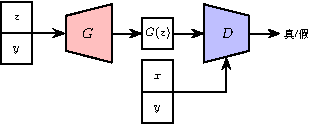
\includegraphics[width=0.8\textwidth]{figures/CGAN.pdf}
	\caption{条件生成对抗网络示意图。图片来自文献~\cite{mirza2014conditional}。}
	\label{fig:pic_CGAN}
\end{figure*}

原始生成对抗网络不能生成具有特定属性的图像结果,针对这个问题,Mirza等人提出条件生成对抗网络(CGAN)~\citep{mirza2014conditional}。如图~\ref{fig:pic_CGAN}所示,核心创新点在于将属性信息$y$融入生成器$G$和判别器$D$中,属性$y$可以是任何标签信息,例如图像的类别信息或者图像本身等。

\subsubsection{DCGAN}
从Alex Krizhevsky等人创造大型深度卷积神经网络AlexNet~\cite{krizhevsky2017imagenet}赢得2012年ImageNet~\cite{deng2009imagenet} 大规模视觉识别挑战赛ILSVRC开始,卷积神经网络(CNN)在计算机视觉领域成功亮相。2016年,Radford等提出了深度卷积生成对抗网络(DCGAN)~\cite{radford2015unsupervised},使用深度卷积神经网络代替原始GAN中全链接层的线性感知,将网络拓展至层数更深、参数更多的任务中,进而提高了生成样本的质量和收敛的速度。

\begin{figure*}[ht]
    \centering
	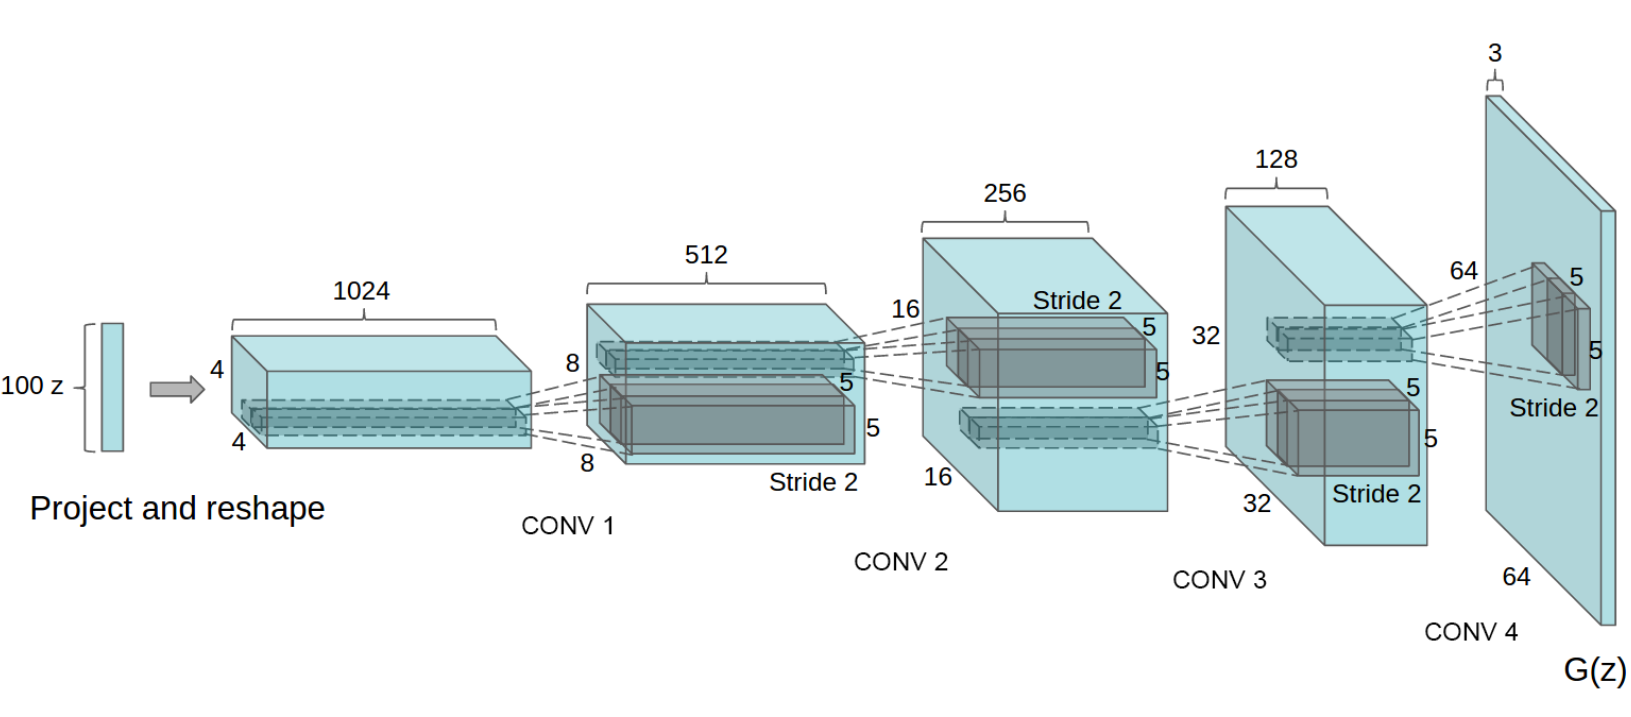
\includegraphics[width=\textwidth]{figures/DCGAN.png}
	\caption{深度卷积生成对抗网络的反卷积过程示意图。图片来自文献~\cite{radford2015unsupervised}。}
	\label{fig:pic_dCGAN}
\end{figure*}

深度卷积生成对抗网络对生成对抗网络的模型结构做了巨大的改进,如图~\ref{fig:pic_dCGAN}所示。创新点如下:(1)在网络结构中取消全链接层,使用全卷积网络。
(2)将对抗网络中的池化层取消,使用带步长的卷积层和反卷积层进行上/下采样操作,更好的提取图像特征。(3)在生成器和判别器中使用批归一化(BatchNorm)~\cite{ioffe2015batch}。
(4)生成器中,除了最后一层使用Tanh激活函数外,其余都是ReLU~\cite{nair2010rectified}激活函数。(5)在判别器中,所有层都使用LeakyReLU~\cite{xu2015empirical}激活函数,从而防止梯度稀疏。

\section{基于生成对抗网络的图像翻译}
图像翻译旨在通过设计端到端的模型将源域图像转换到目标域图像,通常源域提供图像的内容,目标域提供图像的“风格”(可以是图像属性或图像风格),在源域内容下实现目标域的“风格”化,从而实现源域图像到目标域图像的转换。根据训练中是否需要成对图像即源域图像和目标域图像是否一一对应,可以分为成对图像翻译和非成对图像翻译。

\subsection{成对图像翻译方法}

\begin{figure*}[htp]
    \centering
	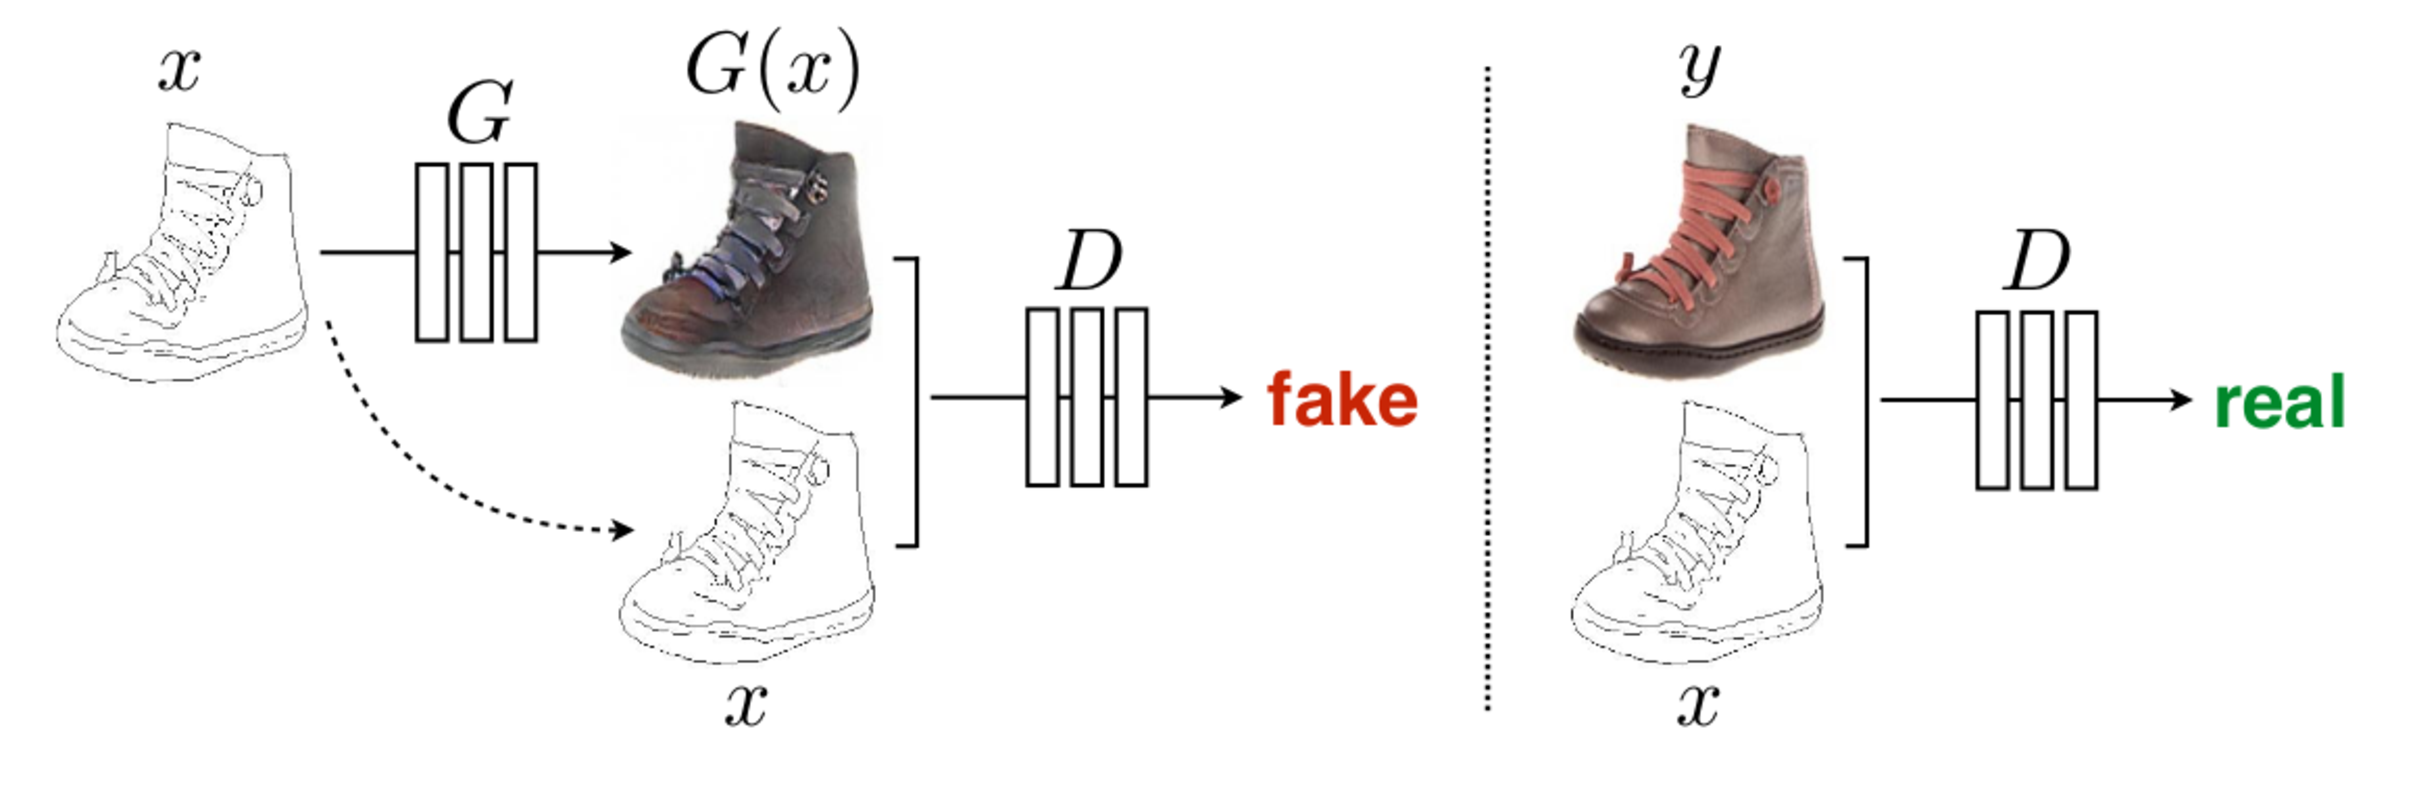
\includegraphics[width=\textwidth]{figures/pix2pix.pdf}
	\caption{pix2pix训练示意图。图片来自文献~\cite{isola2017image}。}
	\label{fig:pix2pix}
\end{figure*}

2017年Isola等人~\cite{isola2017image}提出pix2pix,是典型的配对图像翻译方法。训练过程如图~\ref{fig:pix2pix}所示。网络结果基于CGAN,将图片$x$作为条件,$y$是跟$x$配对的真实结果,需要输入生成器$G$和判别器$D$中。判别器试图区分合成图像$\{x,G(x)\}$和真实图像$\{x,y\}$,生成器试图生成具有真实性的结果以迷惑判别器。生成器采用U-Net全卷积结构,编码过程中对应的特征图和解码之后同样尺寸的特征图按照通道拼接在一起,目的是用来保留不同分辨率下像素级的细节信息。为了更好的对图像局部做判断,判别器利用马尔可夫性的判别器PatchGAN结构。其工作原理是将图像中独立的$N \times N$个patch真假判别,而非将整个图像真假判别,这种设计使得参数更少、运行更快,且能够产生更为锐利的结果。

DRPAN~\cite{wang2019discriminative}针对图像翻译中的高质量高分辨率合成问题,创新性的提出了一种基于块的判别 区域候选机制DRPnet,并构建了一个DRPAN生成对抗网络框架改善合成图像质量,可以得到更高 分辨率、具有更真实细节且更少伪影的高质量图像。所提出的DRPnet机制分别在配对模型pix2pixHD~\cite{wang2018high}和非配对模型CycleGAN~\cite{zhu2017unpaired}上都有很好的泛化能力。

\begin{figure*}[ht]
    \centering
	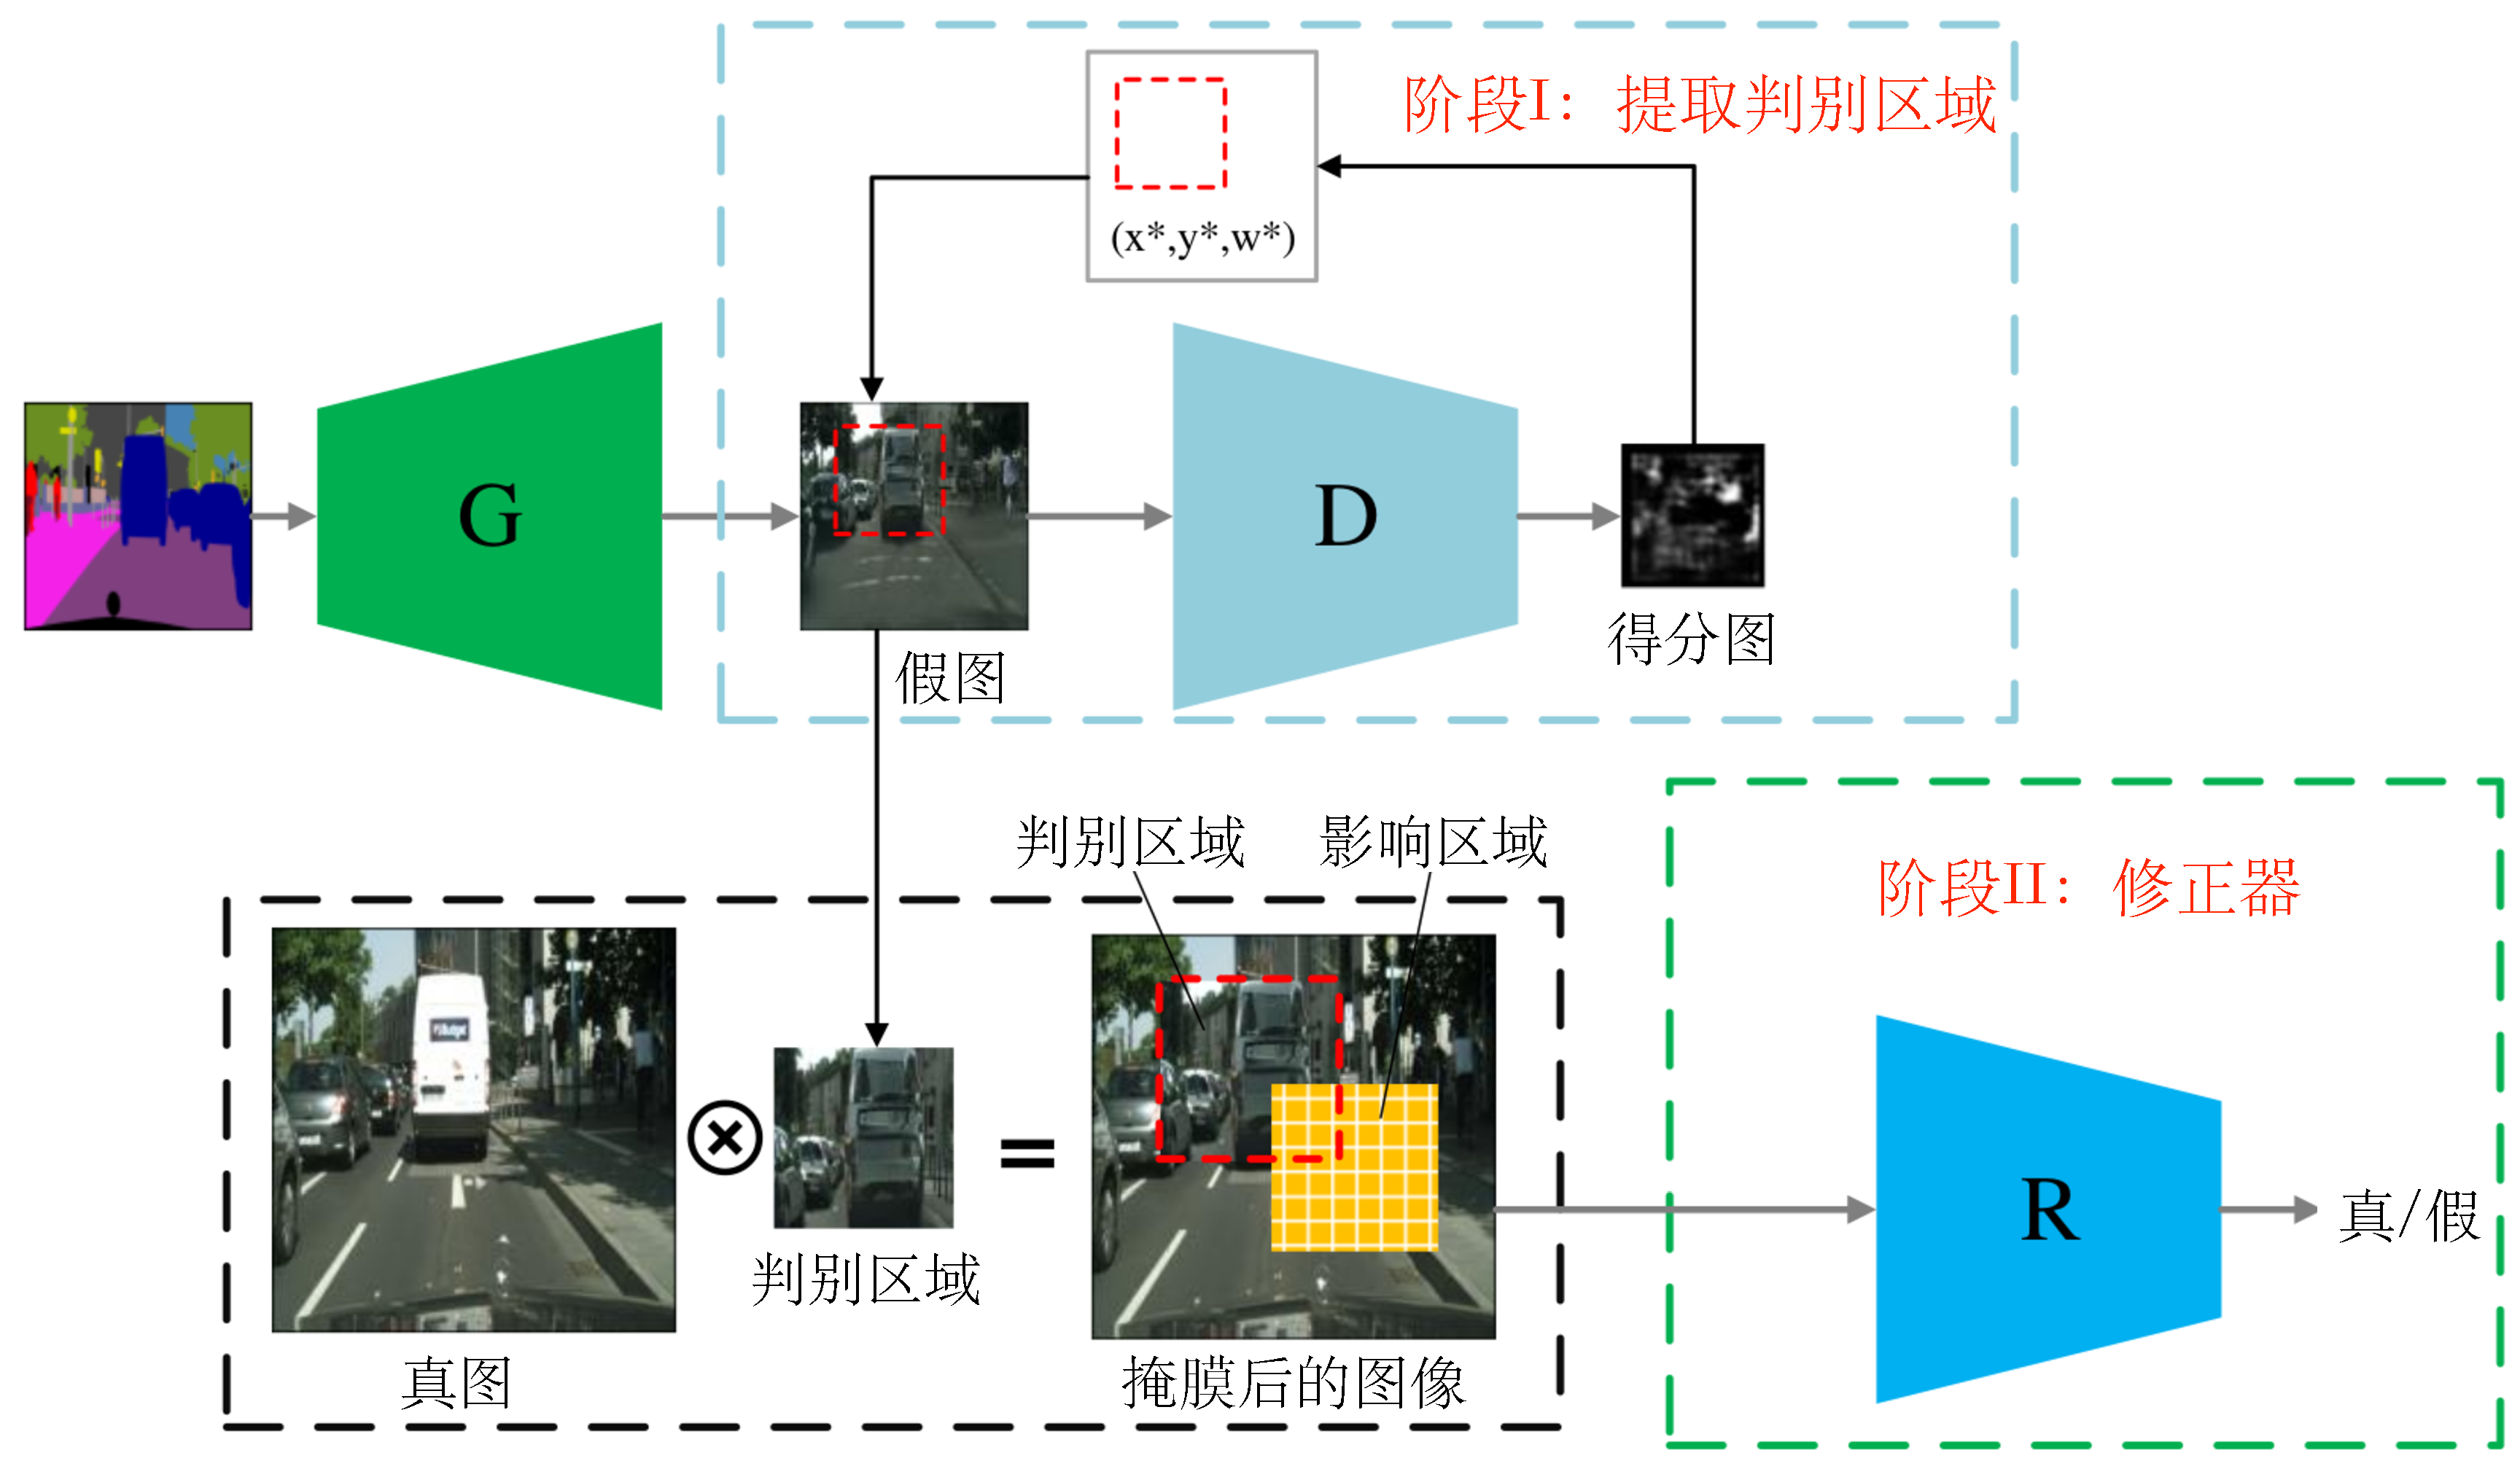
\includegraphics[width=\textwidth]{figures/DRPAN.pdf}
	\caption{DRPAN训练示意图。图片来自文献~\cite{wang2019discriminative}。}
	\label{fig:drpan}
\end{figure*}

\subsection{非成对图像翻译方法}
很多任务中,由于真实数据限制,我们无法得到成对的源域和目标域图像来进行训练,比如将照片翻译成艺术作品风格、人脸翻译成漫画风格等源域和目标域图像没有关联性甚至毫不相干的风格转换任务。由此可见,非成对图像翻译应用场景更加广泛。

\begin{figure*}[ht]
    \centering
	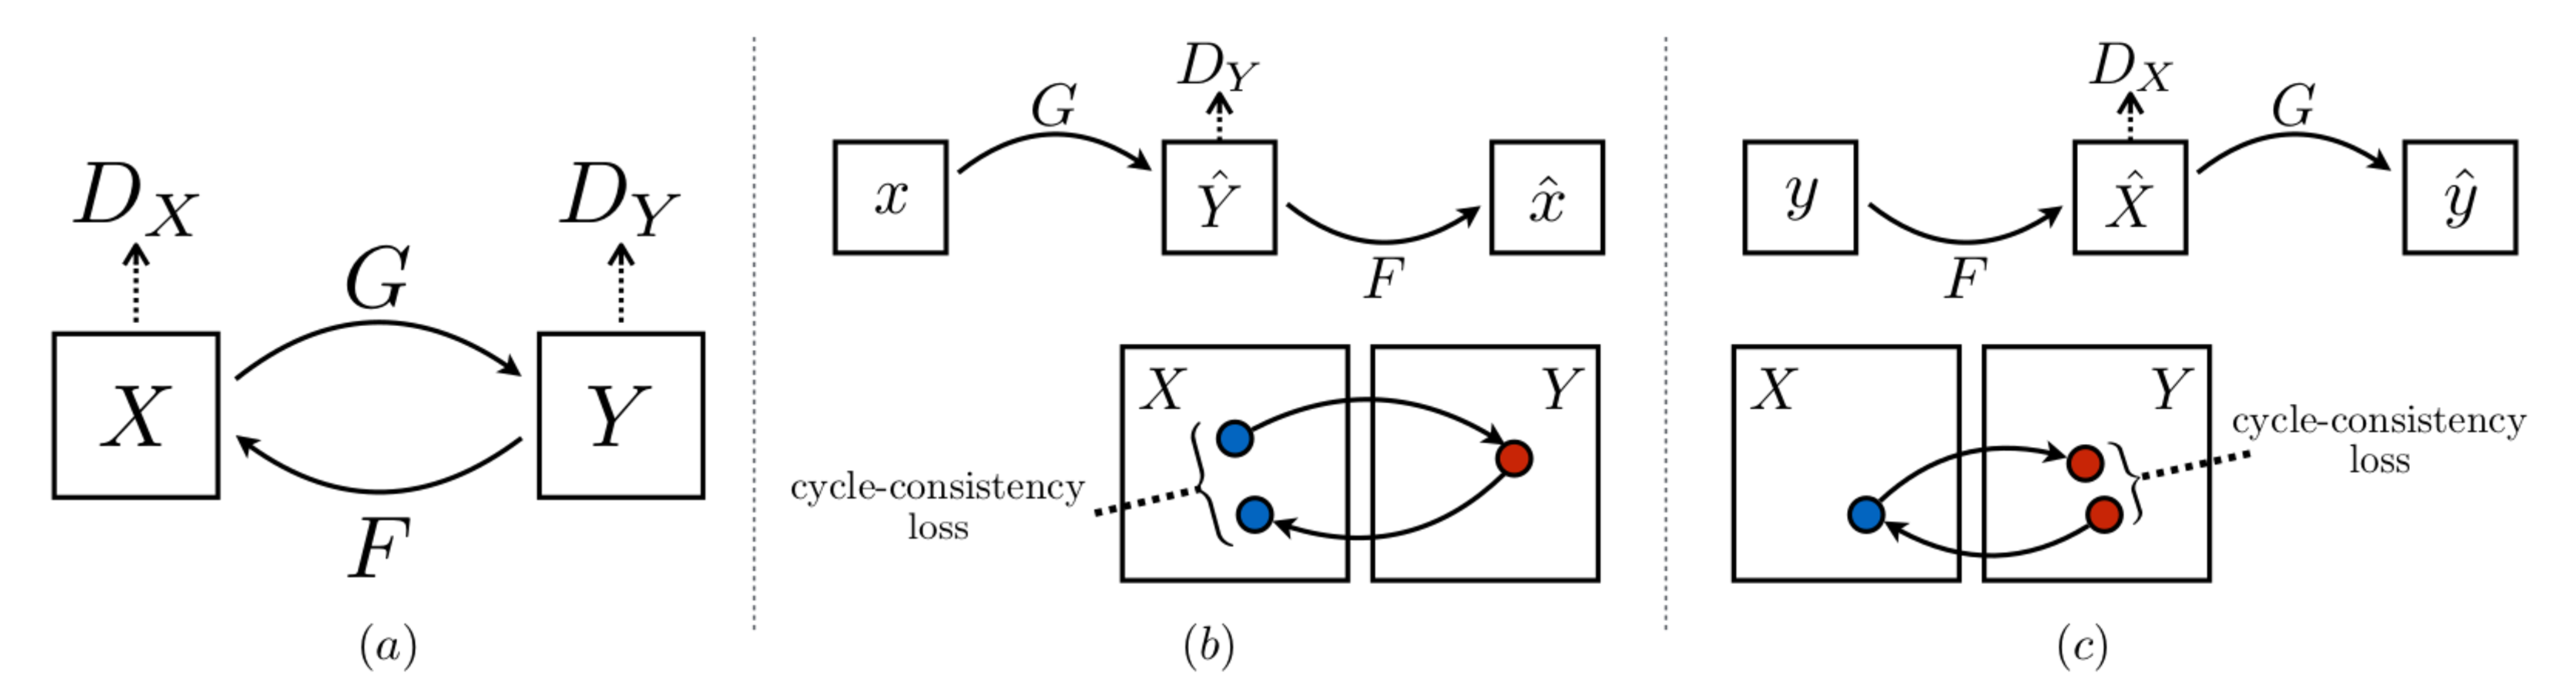
\includegraphics[width=\textwidth]{figures/cyclegan.pdf}
	\caption{CycleGAN训练示意图。图片来自文献~\cite{zhu2017unpaired}。}
	\label{fig:cyclegan}
\end{figure*}

CycleGAN~\cite{zhu2017unpaired}是一种新颖的非配对循环生成结构,主要思路是训练两对生成器和判别器模型将图像从一个域转换到另一个域,过程中要求循环一致性。实质上,CycleGAN在每个方向上都是单向GAN,共享两个生成器,各自带一个判别器,总共两个生成器两个判别器。网络结构如图~\ref{fig:cyclegan}所示,假设有$X$和$Y$两个域,生成器$G$基于$X$域图像生成$Y$域图像;生成器$F$基于$Y$域图像生成$X$域图像,这两个生成器是相反的过程,通过图~\ref{fig:cyclegan}(b)(c)中的循环一致性损失进行约束。CycleGAN的两个判别器$D_X$和$D_Y$分别用来判断输入$X$和$Y$域的图像真假。CycleGAN创新提出的循环一致性损失函数。映射$ G(F(y)) \approx y$和$ G(F(x)) \approx x$在训练过程中学习到。也就是$X$域图片翻译到$Y$域中,还能再逆转回来。

\subsubsection{图像多模态翻译}
从UNIT~\cite{liu2017unsupervised}以共享潜在空间为假设看成图像求联合概率分布,实现非配对的两个域之间分解表达的图像翻译。包括UNIT在内,当时图像翻译无论是配对还是非配对方法,大都是一对一,即输入一张图像只能生成一种风格,缺乏生成结果多样性。比如,同一个场景不同光照条件就是一个模式,不仅仅是白天和黑夜风格,也有傍晚、清晨等风格。在UNIT分解表达学习基础上,MUNIT和DRIT进一步提出多模态图像翻译方法。

MUNIT将潜在空间的潜在编码分为内容编码$c$和风格编码$s$。不同域的图像共享内容编码空间$C$而独享风格编码空间$S$。如图~\ref{fig:munit}(a)部分所示,域$X_1$的风格编码空间为$s_1$内容编码空间为$c_1$,域$X_2$的风格编码空间为$s_2$内容编码空间为$c_2$。内容控制图像中低维信息,风格描述图像中高维属性如颜色、纹理、样式等。网络架构清晰,两个编码器$E_1$ $E_2$分别生成域$X_1$和域$X_2$的内容编码和风格编码;两个生成器$G_1$ $G_2$分别生成域$X_1$和域$X_2$的图像结果;两个判别器$D_1$ $D_2$分别判别域$X_1$和域$X_2$的图像真假。

\begin{figure*}[ht]
    \centering
	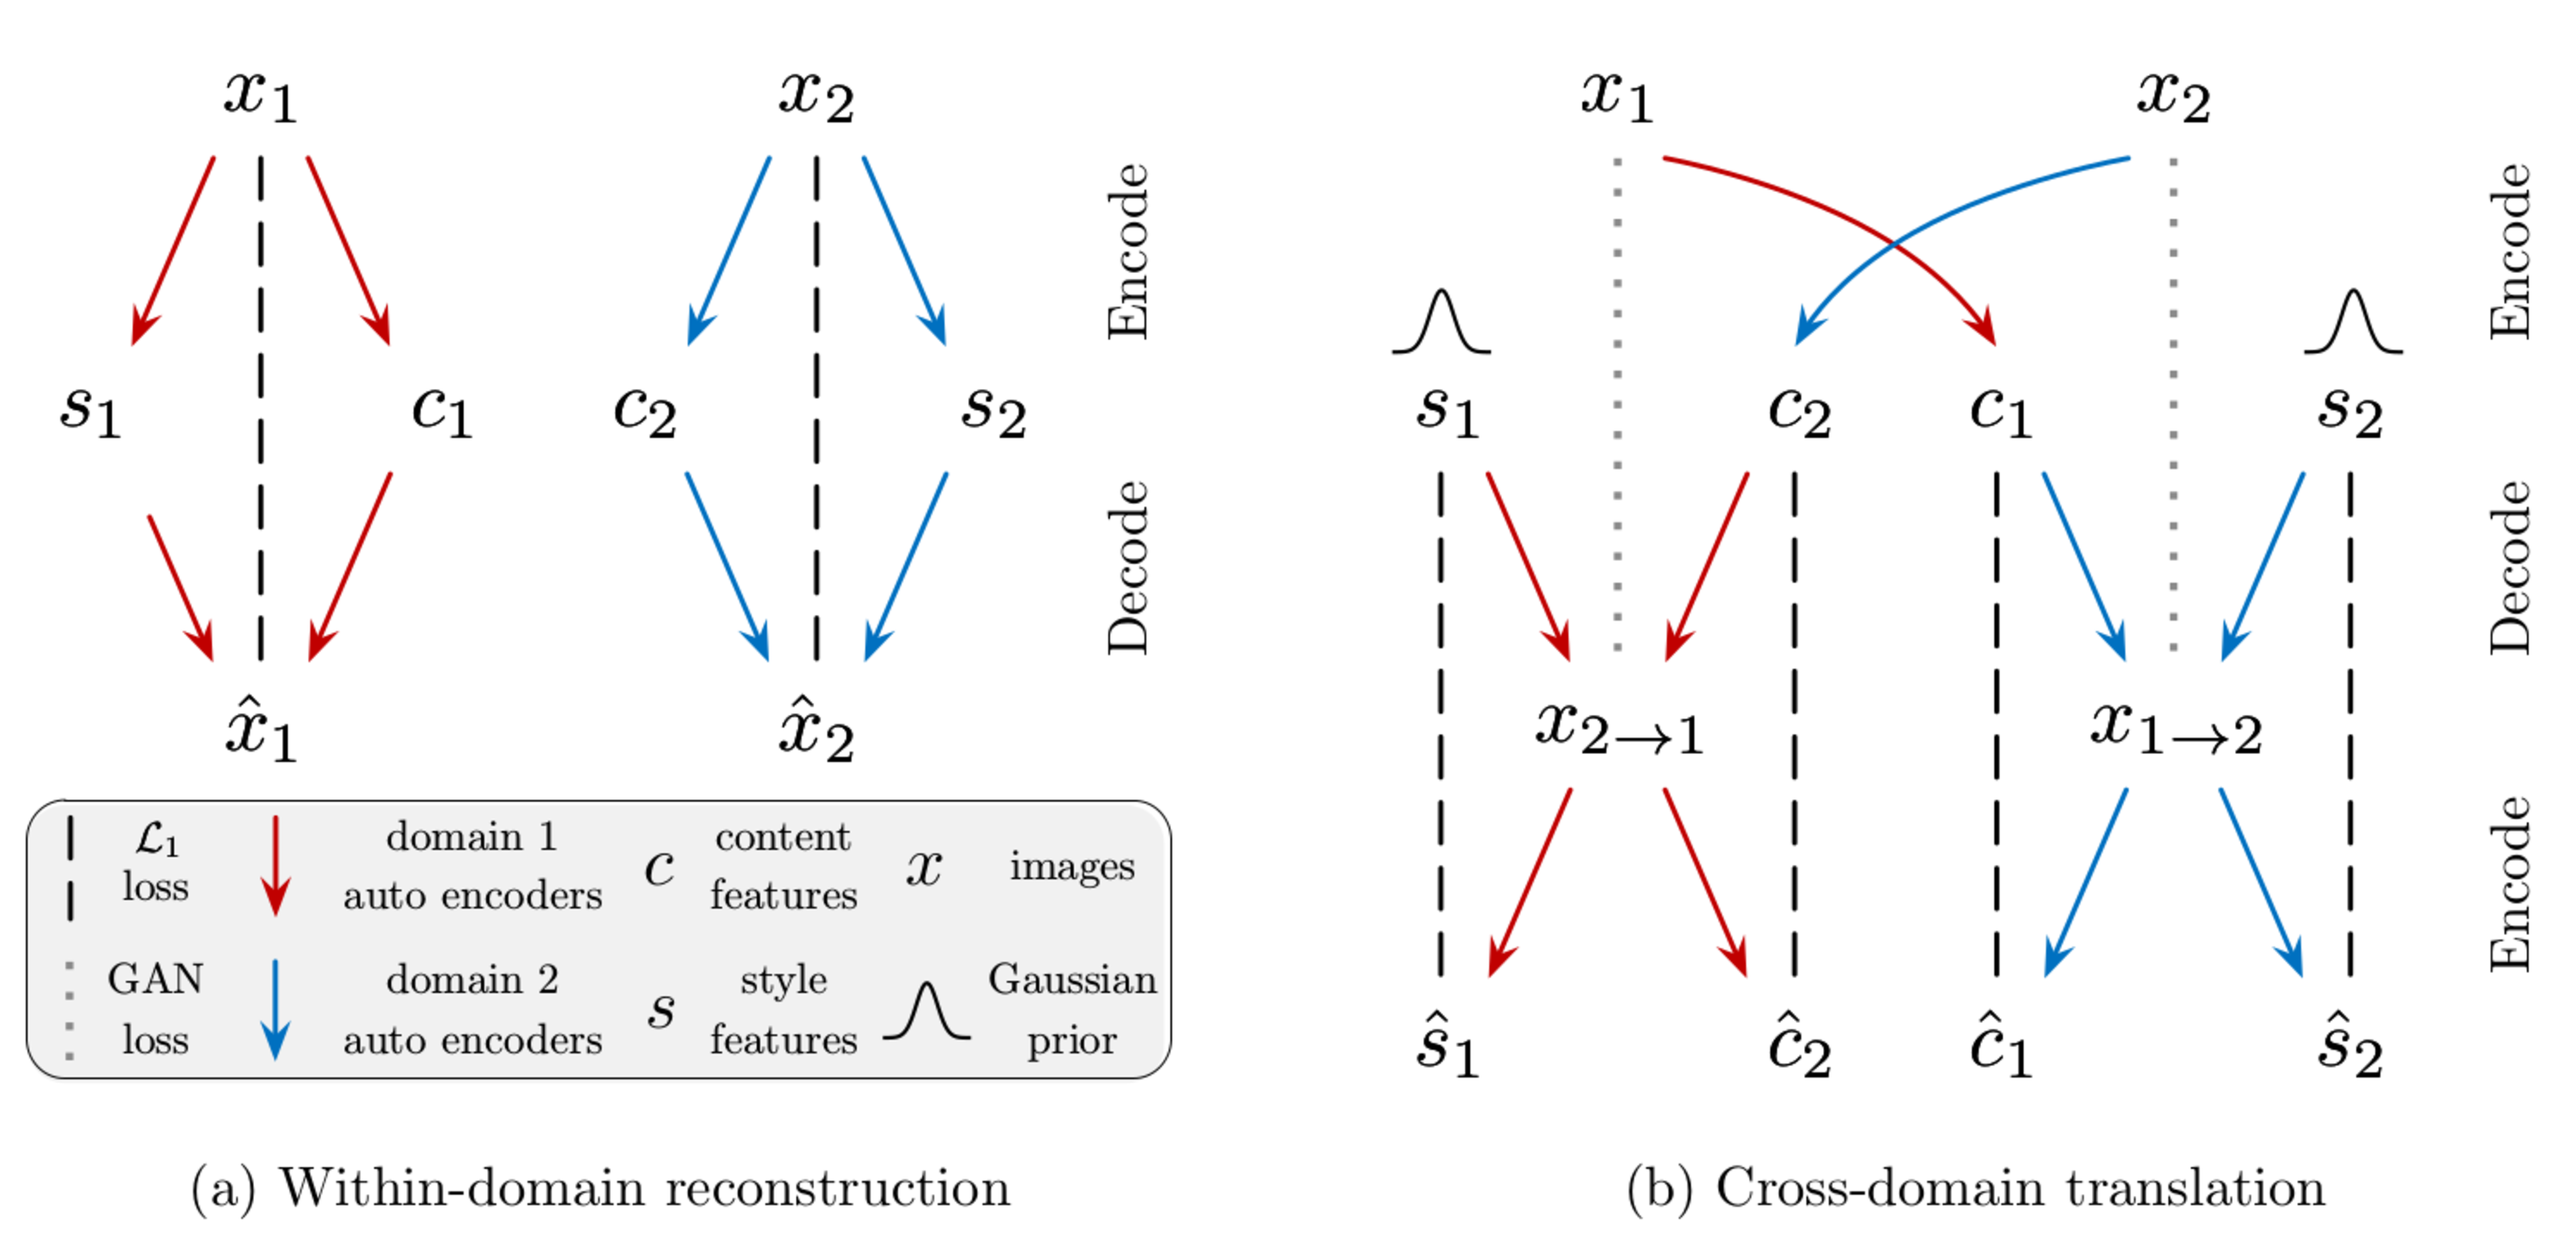
\includegraphics[width=\textwidth]{figures/munit.pdf}
	\caption{MUNIT训练示意图。图片来自文献~\cite{huang2018multimodal}。}
	\label{fig:munit}
\end{figure*}

整个网络的训练包括两个部分,如图~\ref{fig:munit}(a)所示的域内重建和如图~\ref{fig:munit}(b)所示的跨域翻译。MUNIT结构包括生成结构和判别结构,生成结构包括编码器和解码器。编码器包括内容编码器和风格编码器,解码器采用AdaIN~\cite{huang2017arbitrary}仿射变换将目标域风格翻译;判别器使用多尺度判别器~\cite{wang2018high}结构,能帮助实现高分辨率图像的判别。由此,可以构建重建损失函数包括图像重建损失函数,内容重建损失和风格重建损失函数。

DRIT~\cite{lee2018diverse}跟MUNIT在思路上完全一致,都是共享内容空间,独享属性/风格空间。网络训练如图~\ref{fig:drit}所示同样由域内重建和跨域翻译两个部分组成,跨域翻译用来生成交换风格厚的图像,域内重建被编码后的潜在编码。用$X, Y$表示两个域,网络由两个内容编码器$E_{X}^{c}$和$E_{Y}^{c}$和两个属性编码器$E_{X}^{a}$和$E_{Y}^{a}$,两个生成器$G_X$和$G_Y$以及两个判别器$D_X$,$D_Y$组成。其中$u=G_X(E_Y^c(y),E_X^a(x))$,$v=G_Y(E_X^c(x),E_Y^a(y))$。

\begin{figure*}[ht]
    \centering
	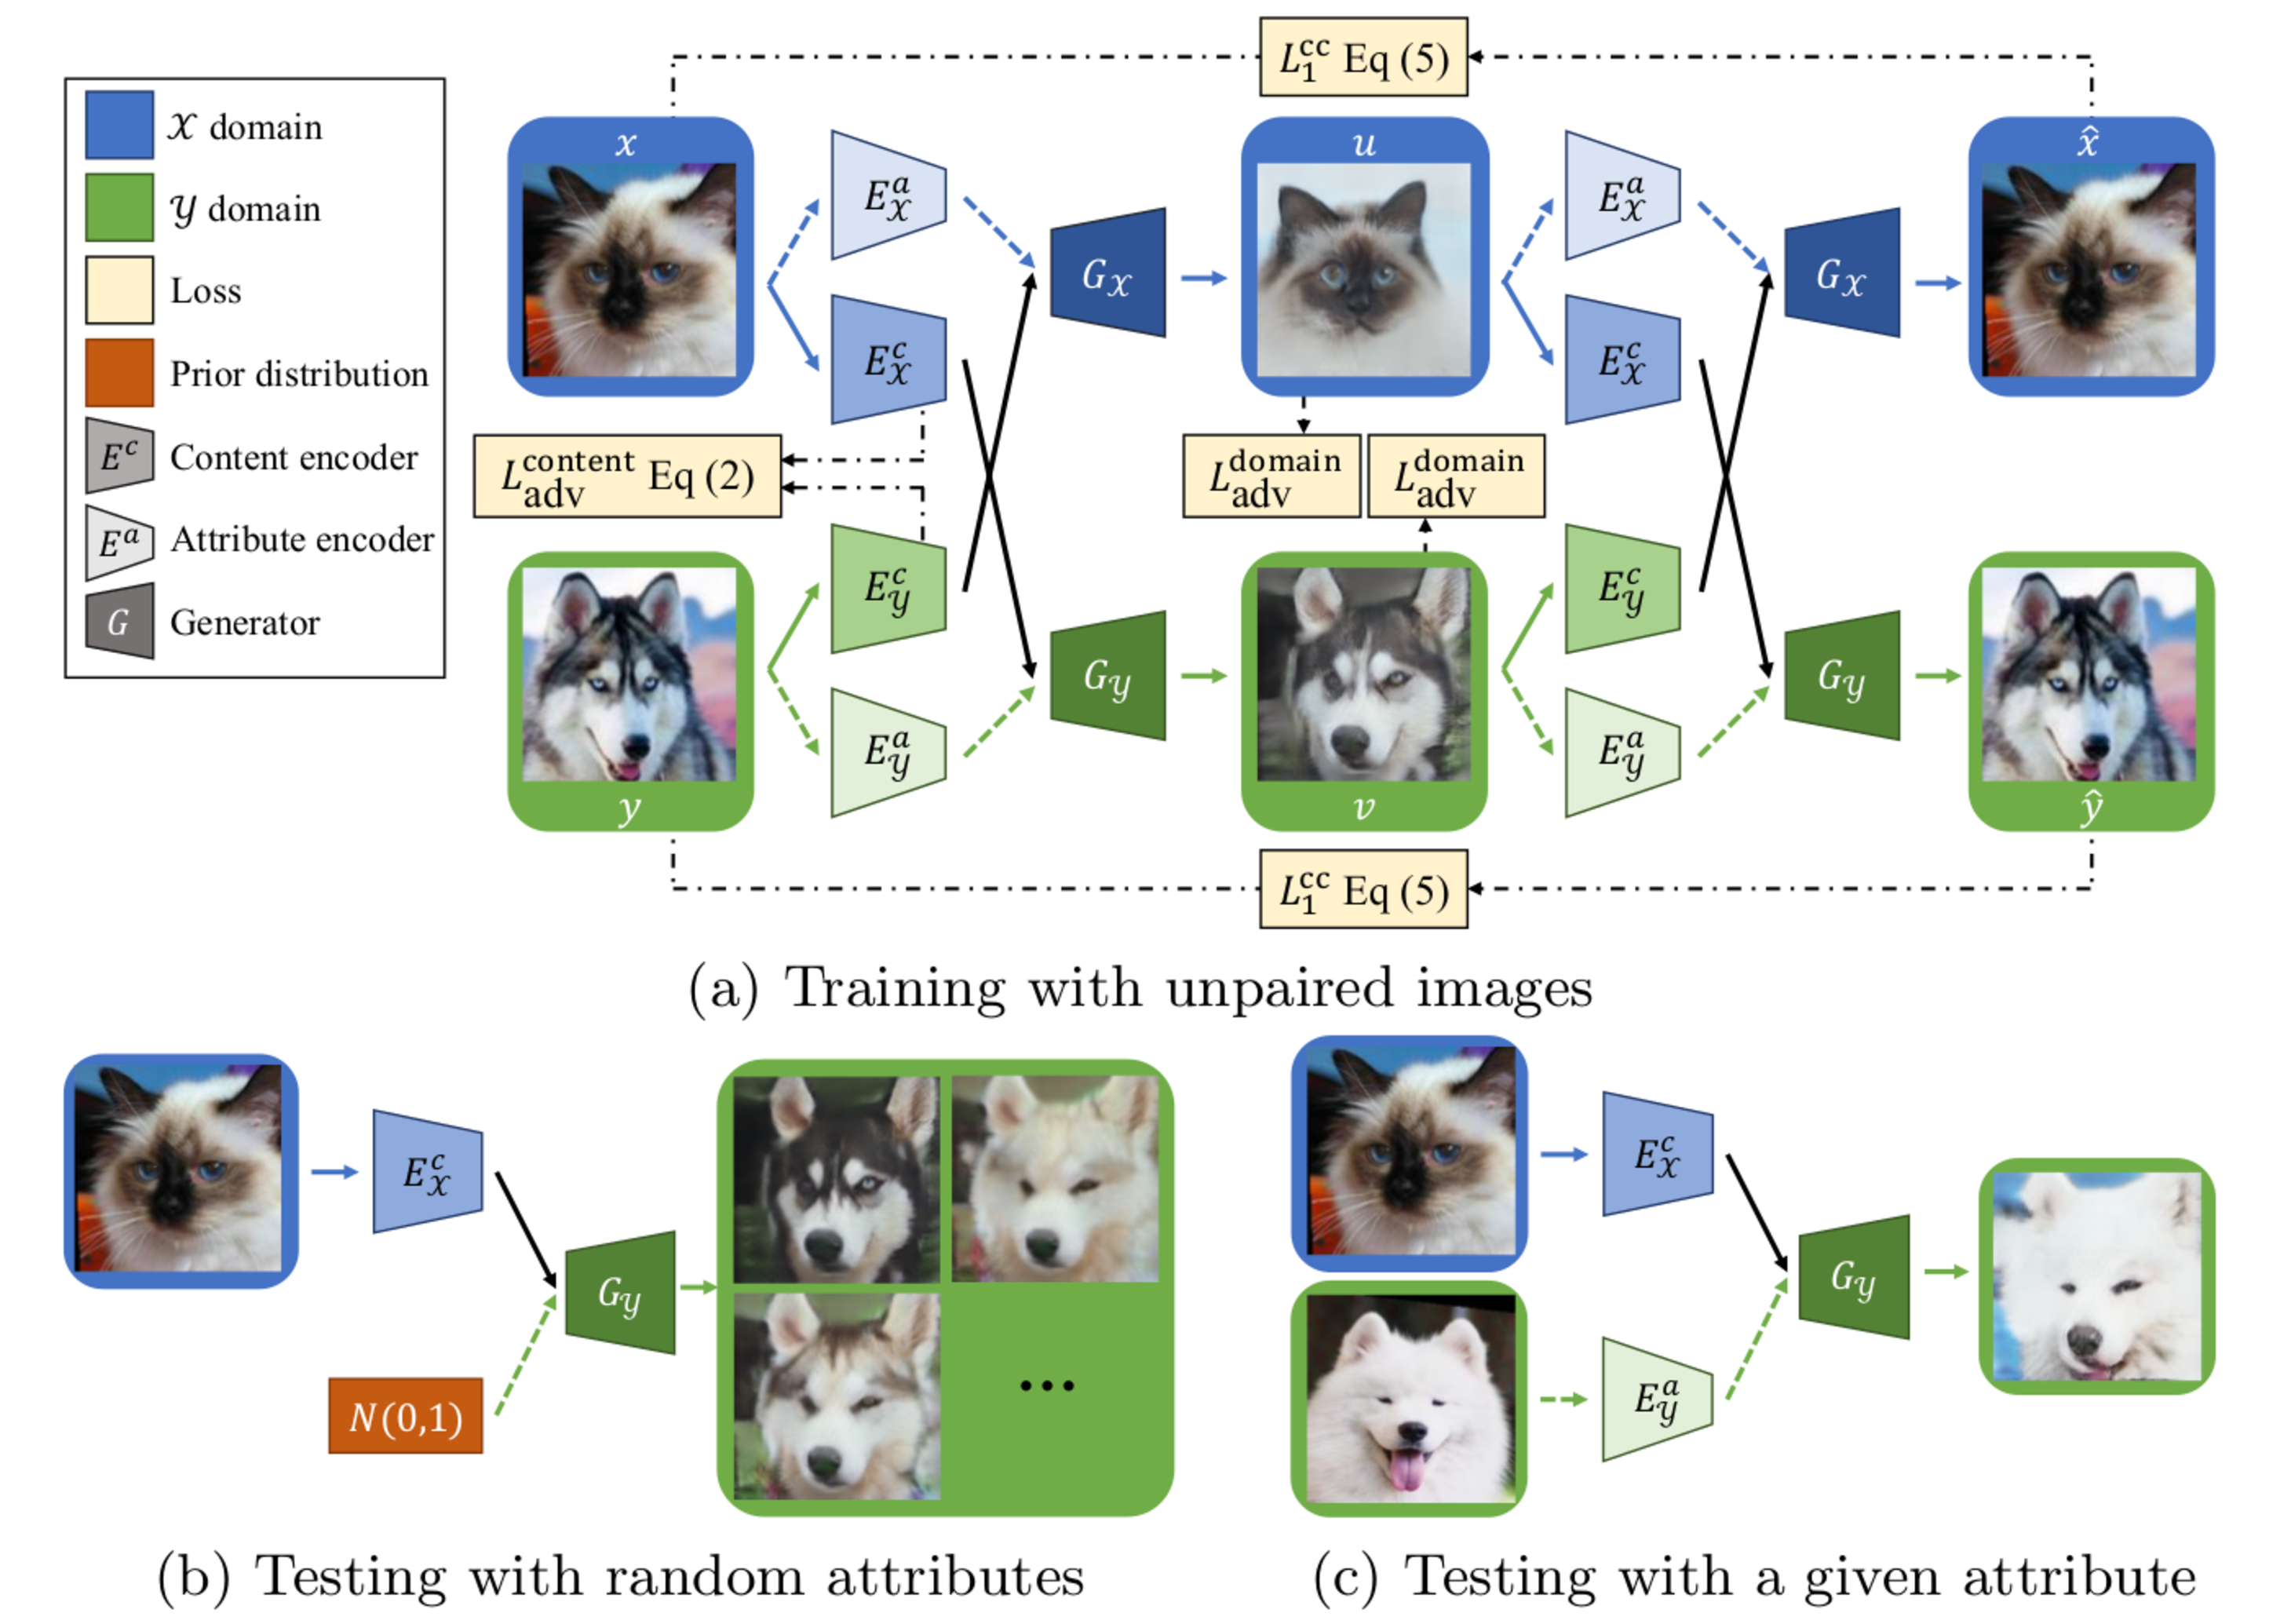
\includegraphics[width=\textwidth]{figures/DRIT.pdf}
	\caption{DRIT训练示意图。图像来自文献~\cite{lee2018diverse}。}
	\label{fig:drit}
\end{figure*}

跨域翻译和域内重建跟MUNIT一致,在此不再赘述。在内容编码和属性编码结合时,DRIT和MUNIT有一定的差异,MUNIT将风格编码使用AdaIN内嵌到生成器(解码器)的中间层,而DRIT采用共享两个编码器$E_X^c$,$E_Y^c$最后一层和两个生成器$G_X$,$G_Y$第一层的权值。

DSMAP~\cite{chang2020domain}基于MUNIT分解表达方式,将图像分解到内容空间和风格空间,但DSMAP认为MUNIT内容空间分解不彻底,DSMAP提出将共享内容空间的特征进行再映射到域特有的内容潜在空间中。经过再一次分解,此时将内容信息再一次净化,得到纯净的域特有内容信息,有助于后续跨域翻译和域内重建的进行。此方法搭建一个更好的图像的内容域和样式域沟通的桥梁,使得最终生成的图像能更好更真实的表达出来。

\begin{figure*}[ht]
    \centering
	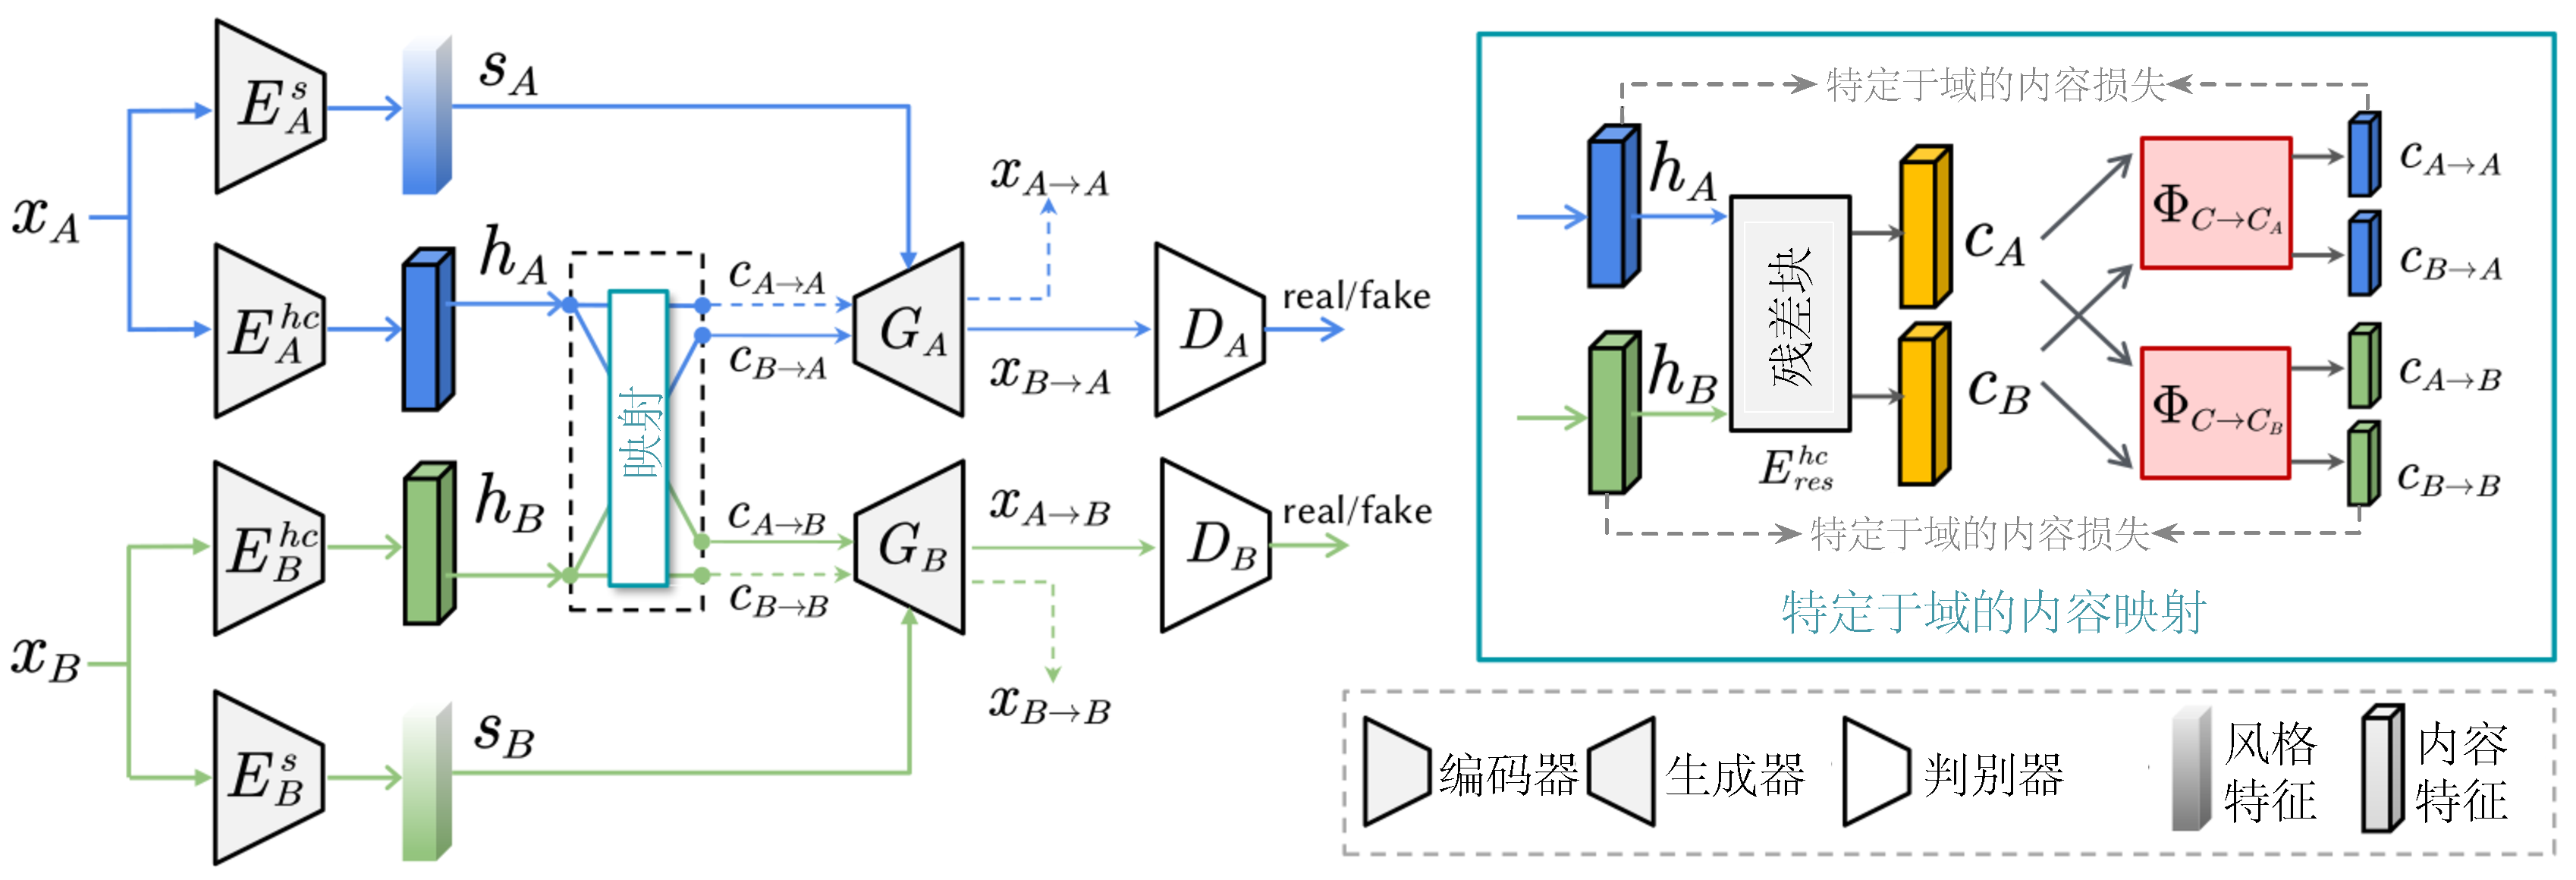
\includegraphics[width=\textwidth]{figures/DSMAP.pdf}
	\caption{DSMAP训练示意图。图像来自文献~\cite{chang2020domain}。}
	\label{fig:dsmap}
\end{figure*}

DRIT++~\cite{lee2020drit++}在DRIT基础上加入Mode Seeking Regulation~\cite{mao2019mode}解决模式崩溃问题并提高生成多模态样式的能力。StarGAN v2~\cite{choi2020stargan}引入映射网络和风格编码器将输入的风格噪声向量和输入风格图像编码到风格潜在空间,通过将随机采样的噪声向量输入生成目标域多模态结果。

\subsubsection{图像多域翻译}

\begin{figure*}[ht]
    \centering
	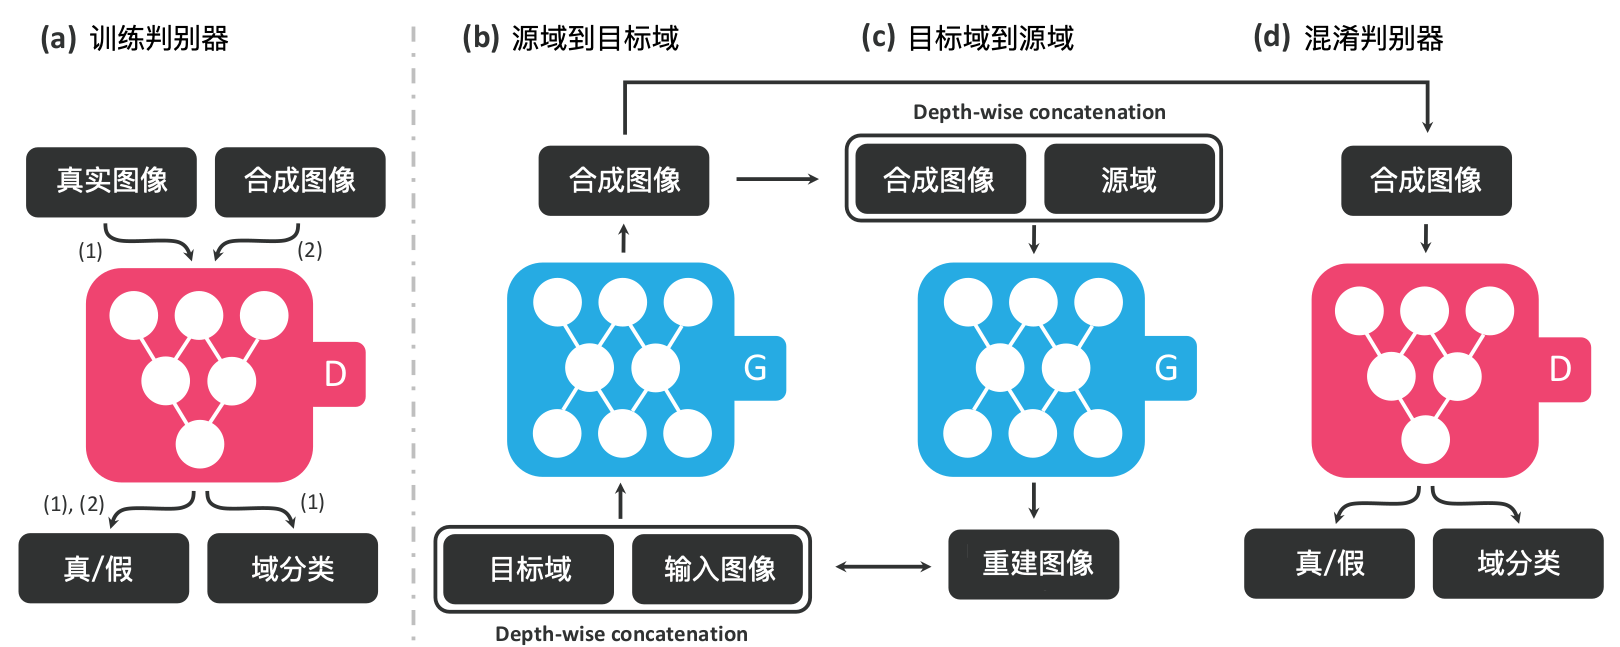
\includegraphics[width=\textwidth]{figures/star.png}
	\caption{StarGAN模型示意图。图像来自文献~\cite{choi2018stargan}。}
	\label{fig:star}
\end{figure*}

如图~\ref{fig:star}所示,StarGAN~\cite{choi2018stargan}将有同一种属性的一组数据作为一个域,对该属性进行属性编码,通过属性编码让生成器学会到多个域的翻译。在生成器的输入中添加目标域编码信息,判别器除了具有判断图片是否真实的功能外,还要有判断图片属于哪个域的能力。这样可以保证生成器中同样的输入图像,随着目标域的不同生成不同的效果。需要保证图像翻译过程中图像内容保存,只改变域间差异的那部分。StarGAN通过图像重建保证内容保持不变,图像重建即将图像翻译从域A到域B,再从域B到域A,此时重建结果与输入结果相比不会发生变化。StarGAN学习每个域的确定性映射,这可能无法获取数据分布的多模式性质。在给定源图像的情况下,它不可避免地在每个域中产生相同的输出。

\begin{figure*}[ht]
    \centering
	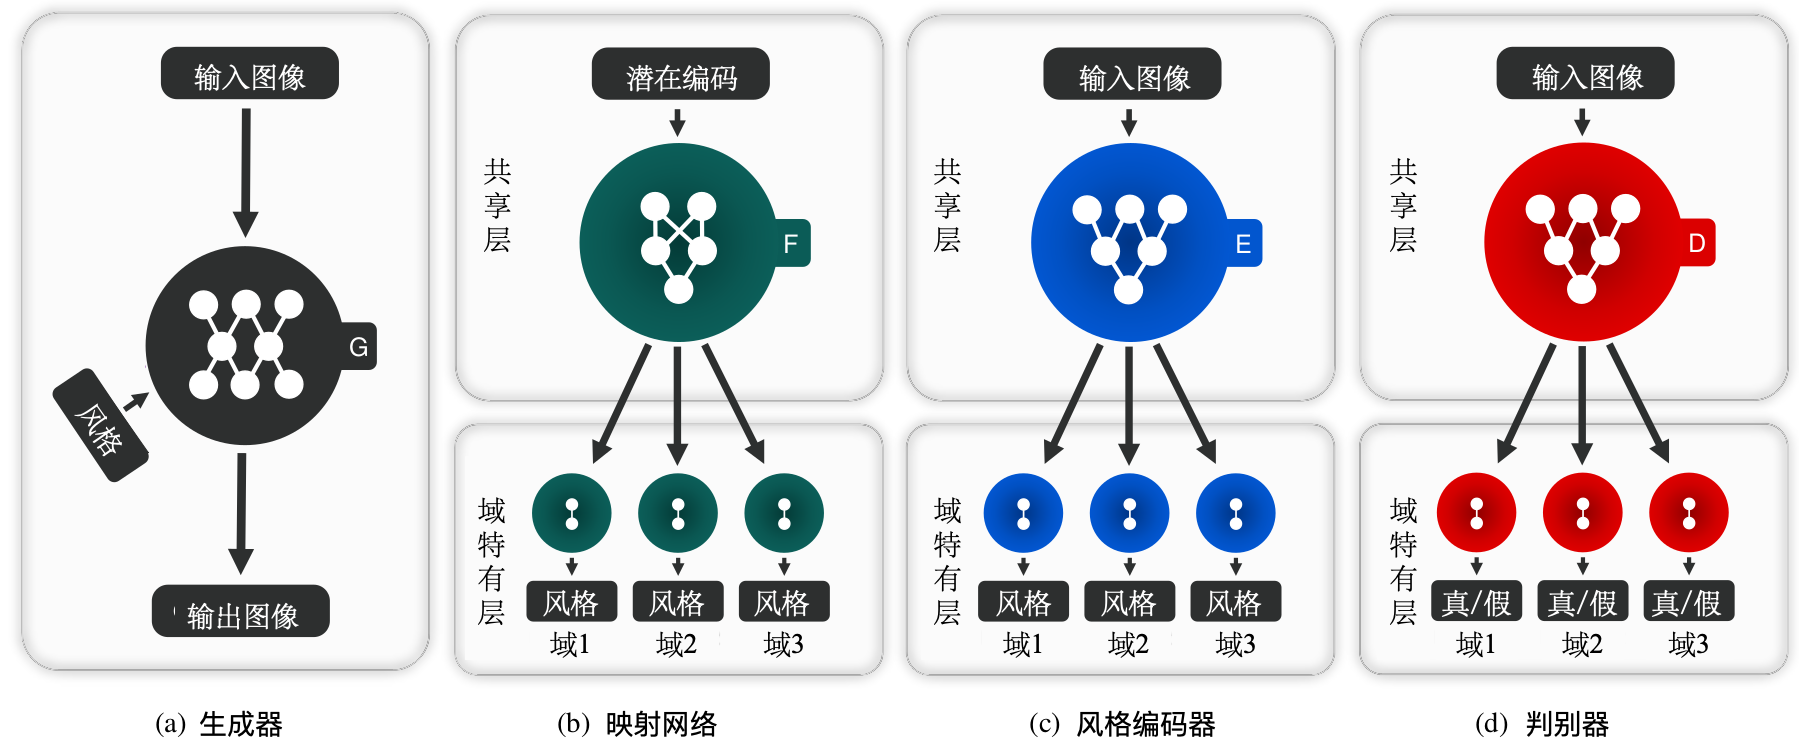
\includegraphics[width=\textwidth]{figures/starv2.png}
	\caption{StarGAN v2模型示意图。图像来自文献~\cite{choi2020stargan}。}
	\label{fig:starv2}
\end{figure*}

如图~\ref{fig:starv2}所示,StarGAN v2~\cite{choi2020stargan}以StarGAN为基础,用特定域的样式代码替换原来的域标签,这些代码可以表示特定域的各种形式。StarGAN v2引入两个模块,一个映射网络和一个样式编码器。前者学习将随机高斯噪声转换为样式代码,后者学习从给定的参考图像中提取样式代码。
StarGAN v2在图像质量、多样性和可扩展性方面与StarGAN和其它基准方法比实现了提升。DRIT++~\cite{lee2020drit++}则是在DRIT两个域多模态翻译任务基础上,通过分解表达用一个生成器进一步实现多域之间翻译。当为多个域的时候,输入其中两个域图像以及对应域内随机采样得到的one-hot编码,用DRIT中同样地的训练方法进行模型训练,将两个域之间的翻译拓展至多个域。

\section{水下图像翻译}\label{sec:underwater}
\subsection{水下图像成像}
水下环境的特殊物理和化学特性严重影响了水下图像的质量和数量,产生许多比在地面成像更难克服的问题。如图~\ref{fig:underwater}所示,水下成像有许多陆地图像不存在的问题。

\begin{figure*}[ht]
    \centering
	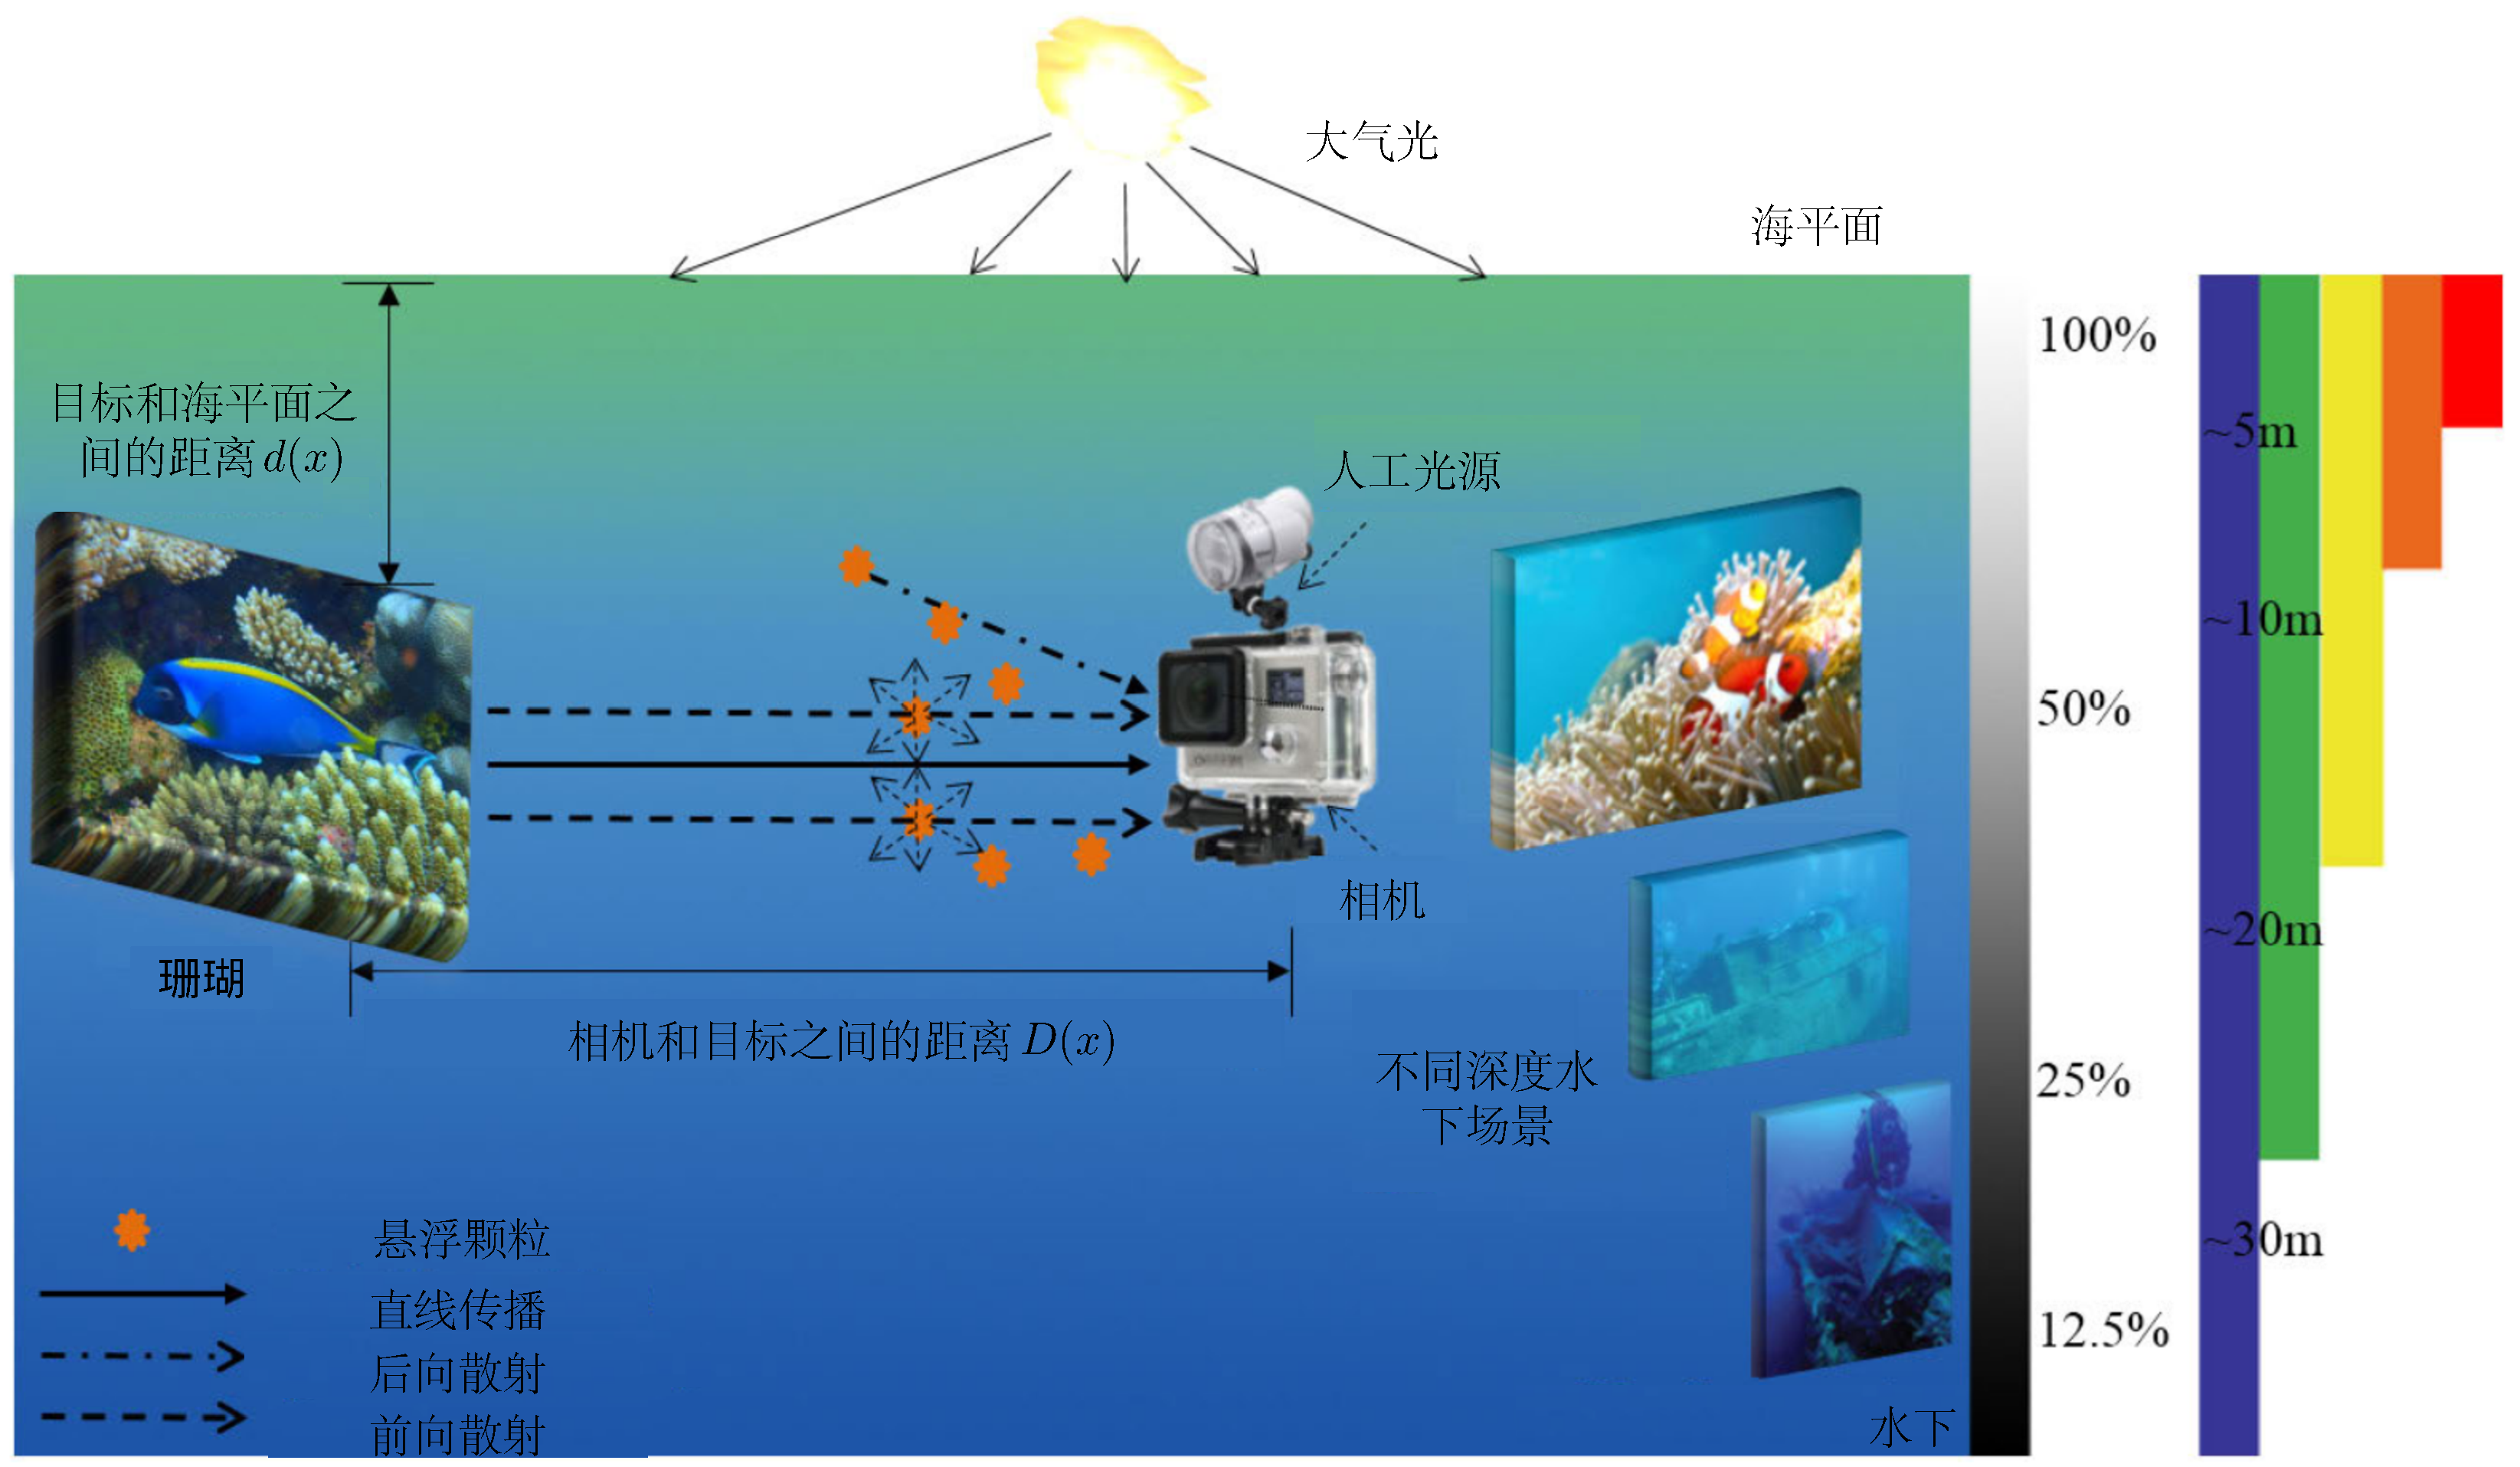
\includegraphics[width=\textwidth]{figures/水下成像.pdf}
	\caption{水下光学成像原理图。图片来自文献~\cite{2002Vision}。}
	\label{fig:underwater}
\end{figure*}

水下图像存在色偏的问题,图像视觉上会呈现蓝色、绿色和蓝绿色。这是由于不同颜色的光在水中的衰减特性造成的,红光波长较长,蓝色和绿色光波长较短,在水介质中光的传播过程中波长较长的光吸收速度更快,因此水下图像都是呈现蓝绿色调。

水下采集到的图像会存在对比度低,模糊等质量下降的问题。吸收和散射是图像降质的原因,即悬浮在水中的颗粒吸收了传播中的大部分光,并将水下场景的反射光在到达相机前改变了光的方向。人为光线除了吸收和散射,还会出现照明不均匀以及照明不足的问题,会造成阴影。

此外,由于水下环境的成像需要耗费巨大的人力和物力资源,水下图像数据量远远小于非水下自然场景的图像数据量,配对的多模态图像结果的获取更难能可贵。缺少水下图像数据给水下视觉研究造成巨大的困难,这也是研究人员针对水下视觉进行大量工作的原因。

\subsection{水下图像翻译}
目前现有的水下图像翻译有两种基本思路。一种是基于深度图和传输图等水下信息加入输入图像中或者基于水下成像衰减模型,使输入图像翻译成具有对应深度或者浑浊度的水下结果。另一种是基于非配对的图像翻译模型CycleGAN,两个域分别是空中图像域和水下图像域,通过循环一致性限制,学习从空中域图像到水下域图像的翻译。

第一种思路有如下工作,每次生成水下图像类型固定,若要生成多样化结果需要训练多个模型依次对应。

WaterGAN~\cite{li2017watergan}用RGB-D~\cite{janoch2013category,lai2014unsupervised,silberman2011indoor,shotton2013scene}的地面图像数据集和水下图像样本集作为输入,使用WaterGAN翻译与RGB-D对齐的相应水下结果,获得成对的结果后在进行水下进一步水下研究。

Underwater-GAN~\cite{yu2018underwater}基于水下成像模型,使用浑浊度模拟器来模拟衰减的水下图像。生成数据集一般需要包括真实图像和对应深度图,在Underwater-GAN中设置相应的散射系数作为深度信息,根据模型计算出散射系数来翻译相对应的水下图像。

UIE-DAL~\cite{uplavikar2019all}和UWCNN~\cite{li2020underwater}使用NYU v2~\cite{silberman2012indoor}数据集中传输图作为衰减系数模拟近海岸和海洋里面不同水类型,控制衰减系数来进行10种水类型的图像翻译。这些方法生成的结果需要依赖于水下信息或者水下,对于真实水下采集到的图像数据缺少泛化能力。

第二种思路有如下工作,使用不成对的数据即可进行水下图像翻译,用非配对图像翻译模型CycleGAN只能实现一对一映射,翻译结果是单模态,缺乏多样性。同样地,要获得多种样式的结果需要多次实现。

UGAN~
\cite{fabbri2018enhancing}此类利用CycleGAN这个非配对一对一映射的图像翻译方法,一个域是空中图像、另一个域是水下图像,通过循环一致来学习从空中到水下图像的翻译。

MLFCGAN~\cite{liu2019mlfCGAN}和Jamadandi等人~\cite{jamadandi2019exemplar}提出的方法等都是用这种方法进行了水下图像翻译,不依赖于任何水下光学模型和任何物理信息。FUnIE-GAN~\cite{islam2020fast}通过相同的方法拓展成包括配对和不配对子集的大规模EUVP数据集。

我们希望通过一个网络模型,仅给定不配对的水下图像数据进行训练,就可以将给定图像同时翻译多种样式的水下结果。为了解决这个问题,可以借鉴我们研究的基于生成对抗网络的非配对图像域翻译的方法,根据水下图像的特点,重新设计相应有效的翻译模型,从而实现将给定图像到多样式水下图像的翻译。这样就可以实现从输入到输出一对多的映射,从而避免需要额外的信息而对数据有较高的要求并限制住模型的泛化能力。

\section{本章小结}
本章深入分析介绍了基于生成对抗网络的图像翻译方法,其中包括如下三个小节。

第一节介绍了生成对抗网络,引入生成对抗网络结构、原理以及目标函数,后续展示了生成对抗网络的发展过程中具有代表性的变种工作。

第二节介绍了基于生成对抗网络的图像翻译,详细讨论了成对图像翻译和非成对图像翻译经典模型,主要是广泛应用的非成对图像翻译基础上的多模态翻译和多域翻译的前沿工作。

第三节介绍了水下图像翻译,首先研究了水下图像的物理模型和成像特点,后分析了水下图像翻译的各种方法,对方法中存在的问题进行了详细的研究和讨论。